\chapter{Caching}

\section{Funzionamento di Base di una Cache}

La memoria principale è sempre stata più lenta di una CPU, questo gap si è ampliato ulteriolmente nel tempo.

\begin{figure}[!h]
    \centering
    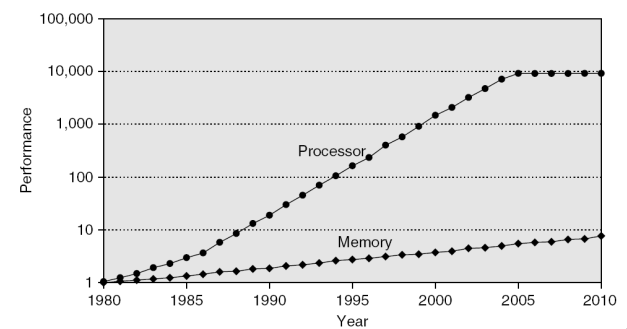
\includegraphics[scale=0.7]{03-Cache/PvsM.png}
    \caption{Andamento nel tempo.}
\end{figure}

\nt{Inoltre la situazione peggiora ancora se si considerano anche i processori multi-core.}

\clm{}{}{
  \begin{itemize}
    \item Il termine SRAM (Static RAM) indica la tecnologia di base con cui sono costruite le RAM usate nei vari livelli di cache del processore. 
    \item Le SRAM usano un circuito di transistor che devono essere sempre alimentati. 
    \item Le DRAM usano un condensatore la cui carica indica se un bit vale 0 o 1. Ogni pochi millisecondi viene fatto un refresh.
    \item Le SRAM sono più veloci, ma consumano di più, sono più complesse e consumano di più.
    \item La cache L1 è ottimizzata rispetto alla velocità di accesso, mentre L2 e L3 rispetto alla capienza di memorizzazione. 
  \end{itemize}
}

\paragraph{Il concetto di caching:}

\begin{itemize}
  \item I registri fanno da cache per la cache hardware. 
  \item La cache hardware fa da cache per la RAM. 
  \item La RAM fa da cache per l'Hard disk (memoria virtuale). 
  \item L'hard disk fa da cache per supporti magnetici più lenti.
\end{itemize}

\dfn{Gerarchi di cache}{
  \begin{itemize}
    \item L1: due cache, una per la data memory  l'altra per la instruction memory. 
    \item L2 e L3 (non in tutti).
  \end{itemize}
}

\begin{figure}[!h]
    \centering
    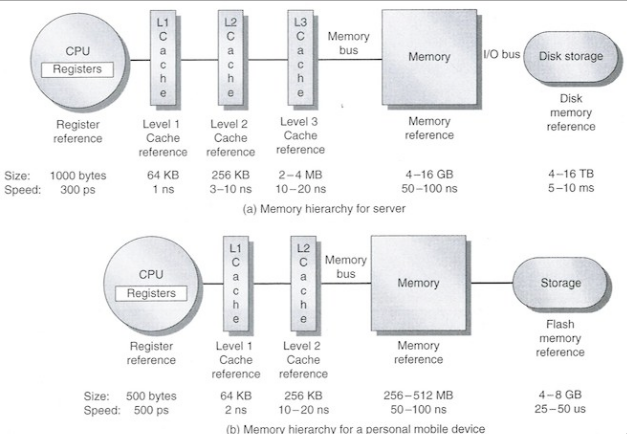
\includegraphics[scale=0.5]{03-Cache/gerarchia.png}
    \caption{Gerarchia di memorie.}
\end{figure}

\cor{Località Spaziale}{
  Area di memoria con indirizzi simili a quelli appena usati, saranno a loro volra usate nell'immediato futuro. 
}

\cor{Località Temporale}{
  Locazioni accedute di recente verranno di nuovo accedute nell'immediato futuro.
}

\dfn{Linee}{Per permettere l’interazione tra memoria cache e RAM, entrambe
sono suddivise in blocchi di dimensione fissa dette linee di cache e
linee di RAM rispettivamente.}

\clm{}{}{
  \begin{itemize}
    \item Ogni linea è identificata dal suo indirizzo in RAM. L'indirizzo in RAM del primo byte appartenente a quella linea.
    \item Il numero della linea dipende dagli m bit più significativi.
  \end{itemize}
}

\cor{Cache Hit}{
  Se viene indirizzata una word che si trova nella cache si ha un cache hit: tutto procede normalmente in quanto la cache è in grado di lavorare alla stessa velocità degli altri elementi del datapath.
}

\cor{Cache Miss}{
  Se viene indirizzata una word che non si trova nella cache si ha un cache miss: il dato viene prelevato dalla RAM e se necessario una linea della cache viene rimossa per fare spazio a quella mancante.
}

\dfn{Cache Direct-Mapped}{
Le cache Direct-Mapped (in italiano: a indirizzamento diretto)
sono il tipo di cache più semplice. Una cache Direct-Mapped è
formata da $2^k$ entry numerate consecutivamente.

Ogni entry memorizza 32 o 64 byte consecutivi e ha associate due informazioni:

\begin{itemize}
  \item Un \textit{bit di validità} che dice se quella entry contiene dell'informazione significativa. 
  \item Un campo \textit{TAG} che identifica univocamente la linea contenuta in quella entry della cache rispetto a tutte le linee della RAM.
\end{itemize}

}
 \nt{In una cache direct-mapped ogni linea della RAM viene memorizzata in una entry ben precisa della cache. Per stabilire in quale entry della cache cercare una linea che contiene il dato o l'istruzione indirizzati dalla CPU si usa l'operazione: (numero della linea in RAM) modulo (numero di entry nella cache).}

\begin{figure}[!h]
    \centering
    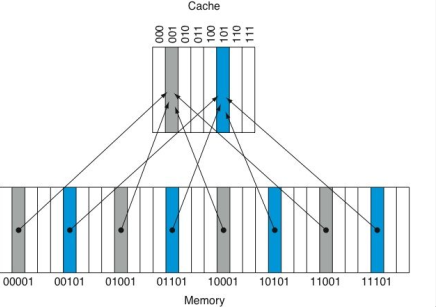
\includegraphics[scale=0.5]{03-Cache/Cache ad accesso diretto.png}
    \caption{Linee di cache.}
\end{figure}




